\documentclass[11pt,a4paper]{article}
\usepackage{amsmath,amssymb,graphicx,booktabs,geometry,xcolor,longtable,array,caption}
\usepackage[colorlinks=true,linkcolor=blue!50!black,urlcolor=blue!50!black,
            citecolor=blue!50!black]{hyperref}
\geometry{margin=2.4cm}
\graphicspath{{../out/}}
\setlength{\parskip}{0.35em}
\captionsetup{font=small,labelfont=bf}

\newcommand{\ad}{\alpha d}
\newcommand{\epsm}{\varepsilon}
\newcommand{\lam}{\lambda}

\title{\bf Physical modelling of Yb:YAG spectroscopic\\ Mueller-matrix data\\[0.4em]
\large Methods, conventions, validation and pitfalls}
\author{Analysis pipeline \texttt{fit/} --- Yb:YAG project, FTMC}
\date{\today}

\begin{document}
\maketitle

\begin{abstract}
\noindent
This document describes, in full, how the refractive index, the Yb$^{3+}$
absorption spectrum and the scattering loss of two Yb:YAG slabs were extracted
from J.\,A.~Woollam RC2 Mueller-matrix data. The analysis replaces an earlier
wavelength-by-wavelength inversion with a single Kramers--Kronig-consistent
oscillator model fitted globally to ten angles of incidence and the
normal-incidence transmittance simultaneously. Emphasis is placed on the parts
that are easy to get wrong: the incoherent treatment of the backside beam, the
Kramers--Kronig partner of the Gaussian oscillator, the fact that the
instrument's own error bars are unusable as fitting weights, the separation of
genuine absorption from instrumental structure, and the decision to fix every
Yb line centre at its predicted Stark-level position rather than fit it. Each
substantive claim is accompanied by the numerical test that supports it.
\end{abstract}

\tableofcontents

\section{Scope and summary}

\subsection{What was measured}

Two uncoated Yb:YAG slabs, labelled A and B, were measured on a J.\,A.~Woollam
RC2 rotating-compensator ellipsometer over $210$--$1700$\,nm:

\begin{itemize}
\item \textbf{Reflection}: the full normalised Mueller matrix at ten angles of
      incidence, $30^\circ$--$75^\circ$ in $5^\circ$ steps (sample B).
\item \textbf{Transmission}: normal-incidence intensity transmittance
      (samples A and B).
\end{itemize}

\subsection{What is extracted}

\begin{enumerate}
\item $n(\lam)$, the refractive index, from the angular dependence of the
      reflection Mueller matrix. This is independent of the slab thickness.
\item The per-pass optical depth $\ad$, split into a Kramers--Kronig-consistent
      \emph{absorption} part carried by Yb$^{3+}$ oscillators and a non-KK
      \emph{scattering} part.
\item The Yb$^{3+}$ oscillator strengths, with line centres fixed at values
      predicted from the crystal-field level scheme.
\end{enumerate}

\subsection{Why a global model rather than point-by-point inversion}

The previous analysis let $n$ and $k$ float independently at each of
$\sim$1000 wavelengths. Two free parameters per wavelength can always reproduce
the data, so the fit was necessarily good --- but it could not answer the
question it raised. The modelled transmittance ran $2$--$3\%$ high in the
near infrared, meaning the loss required to explain $T$ exceeded what $k$ could
carry without spoiling the reflection fit. With $n,k$ free at every point there
is nothing to prevent absorption and scattering trading against each other, and
nothing to identify which is which.

Constraining the whole spectrum to one model closes the trade:

\begin{itemize}
\item the ten-angle reflection Mueller matrix fixes $n(\lam)$ absolutely,
      making no reference to the thickness;
\item the transmittance fixes the \emph{total} per-pass loss
      $(\alpha_{\rm abs}+\alpha_{\rm sc})d$;
\item Kramers--Kronig consistency forbids the absorptive part from taking an
      arbitrary spectral shape --- any $k$ rising towards the NIR must appear in
      $n$ --- so the smooth remainder that cannot be accommodated is pinned as
      scattering.
\end{itemize}

\section{Measurements and file handling}

\subsection{The export format}

The CompleteEASE \texttt{.dat} exports are whitespace-separated, with one
repeating block per (wavelength, angle):

\begin{quote}\ttfamily\small
E \quad $\lam$ \quad $\theta$ \quad $\Psi$ \quad $\Delta$ \quad $\sigma_\Psi$ \quad $\sigma_\Delta$\\
dPolE \quad $\lam$ \quad $\theta$ \quad depol \quad $\sigma$\\
mm11 \quad $\lam$ \quad $\theta$ \quad value \quad $\sigma$ \hfill (raw intensity, $R$ or $T$)\\
mm12 $\ldots$ mm44 \quad $\lam$ \quad $\theta$ \quad value \quad value \quad $\sigma$ \quad $\sigma$ \hfill (normalised to mm11)
\end{quote}

\paragraph{A parsing trap.} The files carry a UTF-8 byte-order mark followed by
CRLF line endings, so the first physical line contains only the BOM and the
\texttt{VASEmethod[\ldots]} header sits on the \emph{second} line. Any parser
that inspects only the first line silently fails to find the header. The reader
opens the files with encoding \texttt{utf-8-sig} and scans all lines for the
header token.

\subsection{Reflection or transmission?}

CompleteEASE writes \texttt{TransmissionMeas=1} into the header for transmission
scans and omits the key entirely for reflection. \textbf{The filename is not
reliable}: \texttt{YbYag\_5a\_MMt} and \texttt{YbYag\_5a\_UMMt} are named with a
trailing ``t'' but carry no transmission flag and were acquired at
$30^\circ$--$75^\circ$, i.e.\ they are reflection scans. The header, not the
name, decides.

\subsection{Data screening}

Every file was screened before use. The results are recorded in the code
(\texttt{SAMPLES} and \texttt{UNUSABLE} in \texttt{run\_fit.py}) so they are not
rediscovered later.

\begin{center}\small
\begin{tabular}{@{}llp{7.6cm}@{}}
\toprule
Sample & Status & Evidence \\
\midrule
B & full $R$ + $T$ fit & reflection at 10 AOI, clean; transmittance clean \\
A & $T$ only & no reflection scan; transmittance clean \\
5\,\% & \textbf{unusable} & transmission files contain \texttt{inf}, negative and
$>1$ values (the entire 2026-06-23 session returned all-NaN); \emph{both} 5a
reflection scans read $m_{12}\!\approx\!0$, $m_{33}\!\approx\!-1$ at
$30^\circ$--$50^\circ$, i.e.\ $\Psi=45^\circ$, $\Delta=180^\circ$, no
polarisation change --- a failed alignment \\
10\,\% & \textbf{unusable} & both transmission files contain negative and $>1$
transmittance; no reflection scan exists \\
\bottomrule
\end{tabular}
\end{center}

A further file, \texttt{YbYag\_B\_UMMt [2026-06-16,175112]}, has median
$T=0.835$, sitting at the lossless-slab limit; it appears to be a
straight-through baseline rather than a sample scan and is excluded.

\paragraph{Both A and B are Yb-doped.} Both show the $940$\,nm pump band at
$\ad\approx0.54$ against a $\approx0.36$ baseline. ``Pure'' in the project
notes means \emph{uncoated}, not undoped.

\paragraph{A physicality filter} is applied to the transmittance: a slab cannot
transmit more than the lossless Fresnel limit
$(1-R_{\rm F})/(1+R_{\rm F})$ nor less than zero, and points outside are
discarded as failed acquisitions.

\section{Optical forward model}

\subsection{Geometry and conventions}

The sample is a plane-parallel slab of complex index $N_1=n+ik$ in air
($N_0=1$), of thickness $d$ in the millimetre range. The time convention is
$e^{-i\omega t}$, so a forward-propagating wave carries
$\exp\!\left(i\,2\pi N\cos\theta\, z/\lam\right)$ and $\mathrm{Im}\,N>0$
attenuates.

The refraction angle inside the slab follows from Snell's law with a complex
index,
\begin{equation}
\sin\theta_1=\frac{N_0\sin\theta_0}{N_1},\qquad
\cos\theta_1=\sqrt{1-\sin^2\theta_1},
\end{equation}
where the square-root branch is chosen so that $\mathrm{Im}\cos\theta_1\ge0$;
this keeps evanescent and absorbed waves decaying rather than growing.

\subsection{Fresnel coefficients}

For an interface $a\to b$,
\begin{align}
r_s&=\frac{N_a c_a-N_b c_b}{N_a c_a+N_b c_b}, &
r_p&=\frac{N_b c_a-N_a c_b}{N_b c_a+N_a c_b},\\
t_s&=\frac{2N_a c_a}{N_a c_a+N_b c_b}, &
t_p&=\frac{2N_a c_a}{N_b c_a+N_a c_b},
\end{align}
with $c_a=\cos\theta_a$, $c_b=\cos\theta_b$.

\subsection{From Jones to Mueller}

An isotropic sample has a diagonal Jones matrix $\mathrm{diag}(a_p,a_s)$. Its
(unnormalised) Mueller matrix is
\begin{equation}
\mathbf{M}=
\begin{pmatrix}
\tfrac12(I_p+I_s) & \tfrac12(I_p-I_s) & 0 & 0\\
\tfrac12(I_p-I_s) & \tfrac12(I_p+I_s) & 0 & 0\\
0 & 0 & \mathrm{Re}\,c & \mathrm{Im}\,c\\
0 & 0 & -\mathrm{Im}\,c & \mathrm{Re}\,c
\end{pmatrix},
\label{eq:mueller}
\end{equation}
with $I_p=|a_p|^2$, $I_s=|a_s|^2$ and $c=a_p a_s^{*}$. Written in ellipsometric
angles this is the familiar block-diagonal form
\begin{equation}
\mathbf{M}/M_{11}=
\begin{pmatrix}
1 & -\cos2\Psi & 0 & 0\\
-\cos2\Psi & 1 & 0 & 0\\
0&0& \sin2\Psi\cos\Delta & \sin2\Psi\sin\Delta\\
0&0& -\sin2\Psi\sin\Delta & \sin2\Psi\cos\Delta
\end{pmatrix}.
\label{eq:isoMM}
\end{equation}
Equation~\eqref{eq:isoMM} is the origin of the symmetry relations used in
Sec.~\ref{sec:sym}: $m_{12}=m_{21}$, $m_{33}=m_{44}$, $m_{34}=-m_{43}$.

\subsection{Incoherent superposition of backside beams}

The slab is millimetre-thick and fringe-free at the RC2's spectral resolution.
The front-surface beam and the beams that have made one or more round trips
inside the slab therefore add \textbf{incoherently}: one sums Mueller matrices,
not Jones amplitudes. This is the same physics as CompleteEASE's ``model
backside reflections'' switch, and it is what produces both the measured
depolarisation and the angular fanning of the pseudo-index. Neglecting it makes
the inferred $n$ too low.

Writing $r,t$ for the front face (ambient$\to$substrate), $r',t'$ for the same
face from inside, and $r_b$ for the back face, the $m$-th emergent amplitude is
\begin{equation}
a^{(m)}_{j}=t_j\,t'_j\,r_{b,j}\,\bigl(r_{b,j}r'_j\bigr)^{m-1}\,\beta^{2m},
\qquad j\in\{s,p\},
\end{equation}
where the single-pass amplitude factor is
\begin{equation}
\beta=\exp\!\left(\frac{i\,2\pi N_1\cos\theta_1\,d}{\lam}\right)
      \exp\!\left(-\tfrac12\,\frac{\alpha_{\rm sc}d}{\cos\theta_1}\right).
\label{eq:beta}
\end{equation}
The first exponential carries both the optical phase and the absorption implied
by $\mathrm{Im}\,N_1$; the second carries the non-KK scattering loss introduced
in Sec.~\ref{sec:scatter} (an intensity loss, hence the factor $\tfrac12$ in the
amplitude). The total normalised reflection Mueller matrix is
\begin{equation}
\mathbf{M}_{\rm tot}=\Bigl[\mathbf{M}(r_p,r_s)+\sum_{m=1}^{N_b}
\mathbf{M}\bigl(a^{(m)}_p,a^{(m)}_s\bigr)\Bigr]\Big/ M_{{\rm tot},11},
\end{equation}
with $\mathbf{M}(\cdot,\cdot)$ given by Eq.~\eqref{eq:mueller}. $N_b=3$ round
trips are retained by default; the series converges rapidly because
$|r_b r'|\lesssim0.01$ and $|\beta|^2\approx0.7$.

Because $\mathbf{M}$ depends only on $|a|^2$ and $a_pa_s^*$, the optical phase
in Eq.~\eqref{eq:beta} cancels identically in the sum --- which is precisely the
statement that the beams are incoherent.

\subsection{Transmittance}

For transmission the geometric series can be summed in closed form. Per
polarisation,
\begin{equation}
T_j=\frac{\mathcal{T}_{f,j}\,\mathcal{T}_{b,j}\,A}
         {1-\mathcal{R}_{i,j}\mathcal{R}_{b,j}A^2},
\qquad
A=\exp\!\left(-\frac{4\pi\,\mathrm{Im}(N_1)\,d}{\lam\cos\theta_1}\right)
  \exp\!\left(-\frac{\alpha_{\rm sc}d}{\cos\theta_1}\right),
\label{eq:trans}
\end{equation}
where $\mathcal{T}$ and $\mathcal{R}$ are \emph{intensity} coefficients. The
interface transmittances carry the flux factor
$\mathcal{T}=|t|^2\,\mathrm{Re}(N_b c_b)/\mathrm{Re}(N_a c_a)$. The reported
transmittance is the unpolarised average $\tfrac12(T_s+T_p)$, which at normal
incidence is exact by symmetry.

\subsection{Optional surface roughness}

A nanometre-scale roughness layer, if enabled, is treated \emph{coherently}
(it is far thinner than the coherence length) as a Bruggeman effective medium of
$50\%$ void in the substrate material,
\begin{equation}
f_1\frac{\epsm_1-\epsm_e}{\epsm_1+2\epsm_e}
+f_2\frac{\epsm_2-\epsm_e}{\epsm_2+2\epsm_e}=0 ,
\end{equation}
solved on the branch with $\mathrm{Im}\,\epsm_e\ge0$. The three-phase
ambient/roughness/substrate stack gives effective front coefficients
\begin{equation}
r_{012}=\frac{r_{01}+r_{12}e^{2i\beta_r}}{1+r_{01}r_{12}e^{2i\beta_r}},
\qquad
t_{012}=\frac{t_{01}t_{12}e^{i\beta_r}}{1+r_{01}r_{12}e^{2i\beta_r}},
\end{equation}
which then enter the incoherent slab sum in place of the bare Fresnel
coefficients. Setting $d_{\rm rough}=0$ reduces these identically to the bare
interface. In the final fits roughness is held at zero: $n$ already matches the
single-crystal reference to $0.0018$ without it, so there is nothing for it to
absorb.

\subsection{Validation of the forward model}
\label{sec:slabtests}

\texttt{python fit/slab.py} runs four independent checks:

\begin{center}\small
\begin{tabular}{@{}lll@{}}
\toprule
Test & Expected & Measured \\
\midrule
Lossless slab, normal incidence & $T+R=1$ & exact to $10^{-6}$ printed \\
Isotropy of the reflection MM & $m_{12}\!-\!m_{21}=0$ & $0$ (identically) \\
& $m_{33}\!-\!m_{44}=0$ & $0$ \\
& $m_{34}\!+\!m_{43}=0$ & $0$ \\
Opaque limit $\to$ single interface & $m_{12}=-\cos2\Psi$ & $4.4\times10^{-16}$ \\
& $m_{33}=\sin2\Psi\cos\Delta$ & $2.2\times10^{-16}$ \\
$d_{\rm rough}\to0$ continuity & bare interface & $4.9\times10^{-15}$ \\
\bottomrule
\end{tabular}
\end{center}

\section{Dielectric-function model}

\subsection{Requirement: Kramers--Kronig consistency}

Causality links the real and imaginary parts of $\epsm$,
\begin{equation}
\epsm_1(E)-\epsm_\infty=\frac{2}{\pi}\,\mathcal{P}\!\!\int_0^\infty
\frac{E'\,\epsm_2(E')}{E'^2-E^2}\,\mathrm{d}E' .
\label{eq:kk}
\end{equation}
Enforcing Eq.~\eqref{eq:kk} is what makes the absorption/scattering separation
possible: an absorptive feature cannot be added to $k$ without a corresponding,
measurable signature in $n$.

The model is therefore built entirely from KK-consistent components:
\begin{equation}
\epsm(E)=\epsm_\infty
+\sum_p \frac{A_p}{E_{c,p}^2-E^2}
+\sum_g \mathcal{G}(E;A_g,E_g,\mathrm{Br}_g).
\end{equation}

\subsection{Sellmeier poles and the reference seed}

A pole below the measured range contributes $\epsm_1=A/(E_c^2-E^2)$ with no
absorption. Two are used, one ultraviolet and one infrared, seeded from the
Zelmon single-crystal YAG dispersion~\cite{zelmon},
\begin{equation}
n^2=1+\frac{2.28200\,\lam^2}{\lam^2-0.01185}
      +\frac{3.27644\,\lam^2}{\lam^2-282.734},\qquad [\lam]=\mu\text{m}.
\end{equation}
Conversion to energy space uses
\begin{equation}
\frac{B\lam^2}{\lam^2-C}=\frac{B E_c^2}{E_c^2-E^2},
\qquad E_c=\frac{hc}{\sqrt{C}},
\end{equation}
giving $E_c=11.388$\,eV, $A=296.0\,\mathrm{eV}^2$ for the UV pole and
$E_c=0.07373$\,eV, $A=0.01781\,\mathrm{eV}^2$ for the IR pole. The seed
reproduces the published $n$ to $5\times10^{-6}$ at all test wavelengths, which
verifies the conversion algebra.

\subsection{The Gaussian oscillator and its KK partner}

The Yb$^{3+}$ $4f$--$4f$ lines are inhomogeneously broadened, so a Gaussian
lineshape is appropriate. Its KK partner is analytic in terms of the Dawson
function $D(x)=e^{-x^2}\int_0^x e^{t^2}\mathrm{d}t$. With
$\sigma=\mathrm{Br}/(2\sqrt{\ln2})$,
\begin{align}
\epsm_2(E)&=A\left[e^{-\left(\frac{E-E_g}{\sigma}\right)^2}
                  -e^{-\left(\frac{E+E_g}{\sigma}\right)^2}\right],
\label{eq:gauss2}\\[0.3em]
\epsm_1(E)&=\frac{2A}{\sqrt\pi}\left[
   D\!\left(\frac{E+E_g}{\sigma}\right)-D\!\left(\frac{E-E_g}{\sigma}\right)
   \right].
\label{eq:gauss1}
\end{align}
The second, negative-energy term in Eq.~\eqref{eq:gauss2} enforces the odd
symmetry $\epsm_2(-E)=-\epsm_2(E)$ that Eq.~\eqref{eq:kk} demands; omitting it
biases $\epsm_1$ at low photon energy.

\paragraph{Why not a Lorentzian.} A Lorentzian has $\epsm_2\sim E^{-2}$ wings
that would spread absorption from the $940$\,nm band across the entire
transparent window, where the measurement shows none. The Gaussian's
$e^{-x^2}$ wings vanish far faster and keep the Yb absorption local.

\subsection{Numerical verification of KK consistency}
\label{sec:kktest}

Equations~\eqref{eq:gauss2}--\eqref{eq:gauss1} are verified numerically by
transforming $\epsm_2$ with Eq.~\eqref{eq:kk} on a $4\times10^5$-point grid and
comparing to the analytic $\epsm_1$. The principal value is evaluated by
singularity subtraction, which is exact and remains well behaved \emph{on}
resonance where a naively masked grid does not:
\begin{equation}
\mathcal{P}\!\!\int_0^L\!\frac{x f(x)}{x^2-a^2}\mathrm{d}x
=\int_0^L\!\frac{x f(x)-a f(a)}{x^2-a^2}\mathrm{d}x
+\frac{f(a)}{2}\ln\frac{L-a}{L+a},
\end{equation}
using $\mathcal{P}\int_0^L \mathrm{d}x/(x^2-a^2)=(2a)^{-1}\ln[(L-a)/(L+a)]$.
Agreement is $\sim10^{-10}$ off resonance and $2.4\times10^{-5}$ at the line
centre, the latter limited by grid discretisation. Run with
\texttt{python fit/dispersion.py}.

\subsection{Scattering: a deliberately non-KK channel}
\label{sec:scatter}

A ceramic or defect haze removes light from the specular beam by
\emph{redirecting} it, not by absorbing it. It is therefore not KK-consistent,
and forcing it into $k$ distorts both $n$ and the oscillator strengths. It is
carried separately as an intensity loss with a \textbf{fitted exponent},
\begin{equation}
\alpha_{\rm sc}(\lam)=C\left(\frac{1000\,\mathrm{nm}}{\lam}\right)^{p}.
\label{eq:scat}
\end{equation}

The exponent is fitted rather than fixed at the Rayleigh value $p=4$, and this
matters. The measured loss falls only $\approx20\%$ from $300$ to $1650$\,nm,
whereas $p=4$ would vary by a factor $\sim900$ across that span. A fixed
$\lam^{-4}$ term is consequently driven to zero by the fit and leaves the NIR
transmittance $\approx2\%$ under-predicted --- exactly the discrepancy the
earlier point-by-point analysis reported. The fitted $p$ is thus a diagnostic of
scatterer size, not a nuisance knob.

\section{Yb$^{3+}$ spectroscopy: predicting the line positions}

\subsection{Stark manifolds}

Yb$^{3+}$ has a single excited multiplet. In YAG the crystal field splits the
two manifolds into~\cite{fan}
\begin{align}
{}^2F_{7/2}\ (\text{ground}) &: 0,\ 565,\ 612,\ 785\ \mathrm{cm}^{-1},\\
{}^2F_{5/2}\ (\text{excited}) &: 10327,\ 10634,\ 10927\ \mathrm{cm}^{-1}.
\end{align}
Every allowed electronic absorption line is a difference of one level from each
set, so its \textbf{position is predicted, not fitted}. At room temperature the
$565$, $612$ and $785\ \mathrm{cm}^{-1}$ levels are thermally populated,
producing hot bands to the red of the zero-phonon line (ZPL, $0\to10327$,
$968.3$\,nm).

Boltzmann populations at $300$\,K ($kT=208\ \mathrm{cm}^{-1}$) relative to the
ground level are $0.066$, $0.053$ and $0.023$ for the three excited ground-state
levels, so the hot bands are expected to be weak and the $785\
\mathrm{cm}^{-1}$ ones weakest.

\subsection{Vibronic sidebands}

Phonon-assisted transitions add replicas displaced to the blue of the parent
electronic line by one phonon energy. YAG optical phonons span roughly
$150$--$800\ \mathrm{cm}^{-1}$. Three replicas are included, and they are
\emph{declared as vibronic}, which is what entitles them --- and only them --- to
be broad:
\begin{center}\small
\begin{tabular}{@{}lll@{}}
\toprule
Replica & Displacement & Centre \\
\midrule
ZPL $+150\ \mathrm{cm}^{-1}$   & lowest YAG optical phonon & $954.5$\,nm\\
ZPL $+420\ \mathrm{cm}^{-1}$   & & $930.5$\,nm\\
$10927+500\ \mathrm{cm}^{-1}$  & wing of the $915$\,nm line & $875.1$\,nm\\
$10927+200\ \mathrm{cm}^{-1}$  & & $898.7$\,nm\\
\bottomrule
\end{tabular}
\end{center}

\subsection{Merging unresolved transitions}

Transitions closer than $2$\,nm are merged onto a single intensity-weighted
centre, because the band is not resolved below that separation. Kept separate
they are mutually degenerate: the fit cannot apportion strength between them and
convergence stalls without any gain in information. The threshold must sit below
the $3.2$\,nm spacing of the $965/968/969$\,nm group, which the instrument
\emph{does} resolve --- merging that group leaves $+0.026$ residual on the sharp
ZPL and $-0.011$ on its blue neighbour.

\section{The inverse problem}

\subsection{Observables and isotropy symmetrisation}
\label{sec:sym}

From Eq.~\eqref{eq:isoMM}, an isotropic sample must satisfy $m_{12}=m_{21}$,
$m_{33}=m_{44}$ and $m_{34}=-m_{43}$. The fit therefore uses the symmetric
combinations, which carry all the physical signal:
\begin{equation}
s_{12}=\tfrac12(m_{12}+m_{21}),\quad
s_{33}=\tfrac12(m_{33}+m_{44}),\quad
s_{34}=\tfrac12(m_{34}-m_{43}),
\end{equation}
and reserves the antisymmetric combinations
\begin{equation}
a_{12}=\tfrac12(m_{12}-m_{21}),\ \ \text{etc.}
\end{equation}
for uncertainty estimation, since the model predicts them to be identically
zero.

\subsection{Realistic uncertainties}
\label{sec:errfloor}

\textbf{The instrument's reported error bars cannot be used as fitting weights.}
The RC2 reports $\sigma\sim10^{-4}$ on the normalised Mueller elements and
$\sim6\times10^{-4}$ on transmittance. The true systematic is roughly seventy
times larger, and two independent diagnostics prove it:

\begin{enumerate}
\item $m_{12}-m_{21}$ is consistently $-0.0075$ across all files, although
      isotropy requires the difference to vanish;
\item $\approx10\%$ of measured $m_{12}$ values fall \emph{below} $-1$, which a
      normalised Mueller matrix cannot physically do.
\end{enumerate}

The error assigned to each symmetric observable is therefore
\begin{equation}
\sigma_s=\sqrt{\sigma_{\rm reported}^2+\bigl\langle a^2\bigr\rangle},
\end{equation}
i.e.\ the reported value added in quadrature with the RMS of the corresponding
antisymmetric combination --- a direct, model-free measurement of the instrument
systematic. Transmittance receives a $0.5\%$ photometric floor
(\texttt{--t-sys}).

\paragraph{Consequence.} Left at face value the transmittance block outweighs
the entire ten-angle reflection data set by a factor $\sim100$, and $n$ is
sacrificed to chase a systematic: the fit then returns $n(1550\,\mathrm{nm})
=1.73$. With honest floors it returns $1.8081$, against the single-crystal
reference $1.8070$.

\subsection{Block balancing}

Reflection contributes $\sim3\times10^4$ residuals and transmittance
$\sim10^3$. Each block is scaled by $1/\sqrt{N_{\rm block}}$ so that the two
data types contribute comparably regardless of how many points each happens to
contain; a user-settable multiplier \texttt{--w-trans} allows this to be
overridden.

\subsection{Cost function}

The fit minimises
\begin{equation}
\chi^2=\frac{1}{N_R}\sum_{\text{blocks }b}\ \sum_{\lam,\theta}
\left(\frac{s_b^{\rm mod}-s_b^{\rm meas}}{\sigma_{s_b}}\right)^{\!2}
+\frac{w_T}{N_T}\sum_\lam
\left(\frac{T^{\rm mod}-T^{\rm meas}}{\sigma_T}\right)^{\!2}.
\end{equation}

\subsection{Parameterisation, bounds and the fixed centres}

The free parameters are the two pole amplitudes and the UV pole energy, the
scattering pair $(C,p)$, and for each oscillator its amplitude and width.

\textbf{Line centres are fixed}, not fitted. This is the single most important
choice in the analysis. When centres were free, an oscillator drifted onto
whatever residual bump was nearby and parked itself at $955$\,nm with a $52$\,nm
width against its bound --- a ``crystal-field line'' broader than the entire
manifold structure it was supposed to describe. Fixing the centres also makes
the problem tractable: with free centres neighbouring lines are mutually
degenerate and the optimiser needed $697$ function evaluations instead of $45$.

Widths are bounded by \emph{kind}: electronic lines $\le0.025$\,eV, vibronic
sidebands $\le0.100$\,eV. Without this split the fit again parks a very broad
``line'' against its bound and uses it to absorb whatever the line list is
missing.

\subsection{Optimiser}

\texttt{scipy.optimize.least\_squares}, trust-region reflective, with
\texttt{x\_scale=`jac'} to handle the $\sim10^{-5}$ amplitudes and $\sim10^{2}$
pole amplitudes in one vector. The forward model is fully vectorised over the
$[\lam,\theta]$ grid, so one residual evaluation costs a few tens of
milliseconds and the whole fit converges in $45$ evaluations.

\subsection{Detection limit and the prune-and-refit pass}

An oscillator whose amplitude refines to zero has a width with \emph{zero
gradient}. A single such parameter makes the entire Jacobian singular and
returns \texttt{NaN} for \emph{every} uncertainty in the fit. The pipeline
therefore performs a second pass: lines with $A<10^{-7}$ (corresponding to
$\ad\sim3\times10^{-4}$, more than an order of magnitude below the photometric
floor) are dropped and the fit repeated. They are reported as ``not detected''
rather than silently retained.

\subsection{Parameter uncertainties}

One-sigma values come from the Jacobian at the solution,
\begin{equation}
\mathrm{cov}=\bigl(\mathbf{J}^{\!\top}\mathbf{J}\bigr)^{-1}
\frac{2\,\mathrm{cost}}{N_{\rm res}-N_{\rm par}},
\end{equation}
scaled by the residual variance because the weights are relative rather than
absolute standard deviations.

\section{The thickness degeneracy}

A fringe-free thick slab measures only the \emph{product} $\ad$. The thickness
is an input (\texttt{--thickness}, default $1$\,mm), and:

\begin{itemize}
\item $n(\lam)$ is \textbf{independent} of $d$;
\item $k$, all oscillator amplitudes and both scattering coefficients scale as
      $1/d$.
\end{itemize}

The \texttt{alphad\_abs} and \texttt{alphad\_scat} columns of the output CSV are
the thickness-independent quantities and are the ones to quote. Once $d$ is
measured with a micrometer, multiply through once.

\section{Results}

\subsection{Refractive index}

$n$ matches the Zelmon single-crystal YAG dispersion to \textbf{RMS $0.0018$}
(maximum deviation $0.0047$) over $350$--$1650$\,nm --- from a global model, not
a per-wavelength inversion. Fitted dispersion parameters:
UV pole $A=256.0\ \mathrm{eV}^2$ at $E_c=10.640$\,eV; IR pole
$A=0.0018\ \mathrm{eV}^2$.

\begin{figure}[htbp]
\centering
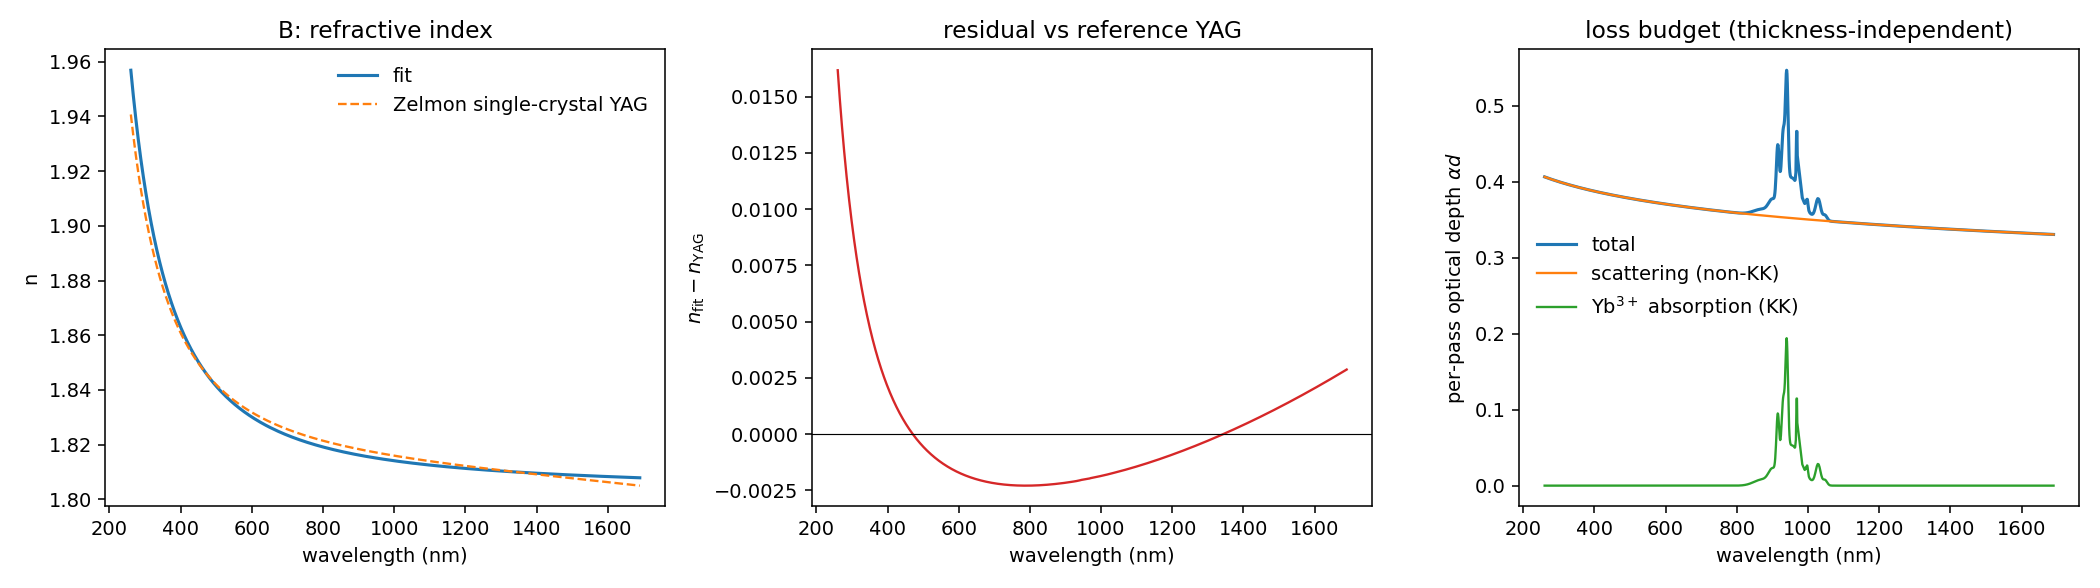
\includegraphics[width=\textwidth]{fig_B_nk.png}
\caption{Sample B. \textbf{Left}: fitted $n(\lam)$ against the single-crystal
YAG reference. \textbf{Centre}: residual, within $\pm0.0025$ across
$400$--$1600$\,nm. \textbf{Right}: the loss budget, separated into the non-KK
scattering channel and the KK-consistent Yb$^{3+}$ absorption. Scattering
accounts for essentially all of the baseline loss; genuine absorption is
confined to the Yb manifold.}
\end{figure}

\subsection{Loss budget}

\begin{equation}
\alpha_{\rm sc}(\lam)=\bigl(3.505\pm0.002\bigr)
\left(\frac{1000\,\mathrm{nm}}{\lam}\right)^{0.1102\pm0.0010}\ \mathrm{cm}^{-1}.
\end{equation}

\textbf{The near-grey exponent $p=0.110$ is the principal physical result.} The
dominant loss in these samples is neither absorption nor Rayleigh scattering: it
is almost wavelength-independent, i.e.\ Mie/geometric scattering from features
comparable to or larger than the wavelength --- grain boundaries and residual
pores. This is what the earlier analysis's unexplained $2$--$3\%$ NIR
transmittance gap actually was. In per-pass optical depth, scattering falls from
$\ad=0.388$ at $400$\,nm to $0.335$ at $1550$\,nm.

\subsection{Yb$^{3+}$ oscillators}

All centres fixed at their predicted positions; only $A$ and the width refine.
Kind ``e'' denotes an electronic Stark transition, ``v'' a vibronic sideband.

\begin{center}\small
\begin{tabular}{@{}rclll@{}}
\toprule
Centre (nm) & Kind & $A$ & FWHM (eV) & Assignment (cm$^{-1}$)\\
\midrule
875.1 & v & $2.10\times10^{-6}\pm3\times10^{-7}$ & 0.100$^\ast$ & $10927+500$\\
898.7 & v & $3.46\times10^{-6}\pm5\times10^{-7}$ & 0.0368 & $10927+200$\\
915.2 & e & $1.92\times10^{-5}\pm9\times10^{-7}$ & 0.0140 & $0\to10927$\\
930.5 & v & $2.11\times10^{-5}\pm8\times10^{-7}$ & 0.0162 & ZPL $+420$\\
\textbf{940.4} & e & $\mathbf{3.72\times10^{-5}\pm1\times10^{-6}}$ & 0.0118 & $0\to10634$ (pump band)\\
\textbf{954.5} & v & $\mathbf{1.46\times10^{-5}\pm4\times10^{-7}}$ & 0.0831 & \textbf{ZPL $+150$}\\
965.1 & e & $1.6\times10^{-6}\pm1\times10^{-6}$ & 0.0020$^\ast$ & $565\to10927$\\
\textbf{968.5} & e & $\mathbf{2.09\times10^{-5}\pm1\times10^{-6}}$ & 0.0040 & $0\to10327$ (ZPL) $+\,612\to10927$\\
993.1 & e & $1.27\times10^{-6}\pm1\times10^{-6}$ & 0.0026$^\ast$ & $565\to10634$\\
997.8 & e & $3.62\times10^{-6}\pm1\times10^{-6}$ & 0.0062 & $612\to10634$\\
1024.4 & e & $1.51\times10^{-6}\pm2\times10^{-6}$ & 0.0191 & $565\to10327$\\
1029.3 & e & $6.89\times10^{-6}\pm2\times10^{-6}$ & 0.0183 & $612\to10327$\\
1048.0 & e & $2.13\times10^{-6}\pm9\times10^{-7}$ & 0.0151 & $785\to10327$\\
\bottomrule
\end{tabular}
\end{center}
{\footnotesize $^\ast$ width at a bound; that parameter's uncertainty is not
meaningful.}

\paragraph{Not detected.} $986.0$\,nm ($785\to10927$) and $1015.3$\,nm
($785\to10634$) refined to zero amplitude and were pruned. Both originate on the
$785\ \mathrm{cm}^{-1}$ level, whose $300$\,K population is only $2\%$, so their
weakness is expected rather than surprising.

\begin{figure}[htbp]
\centering
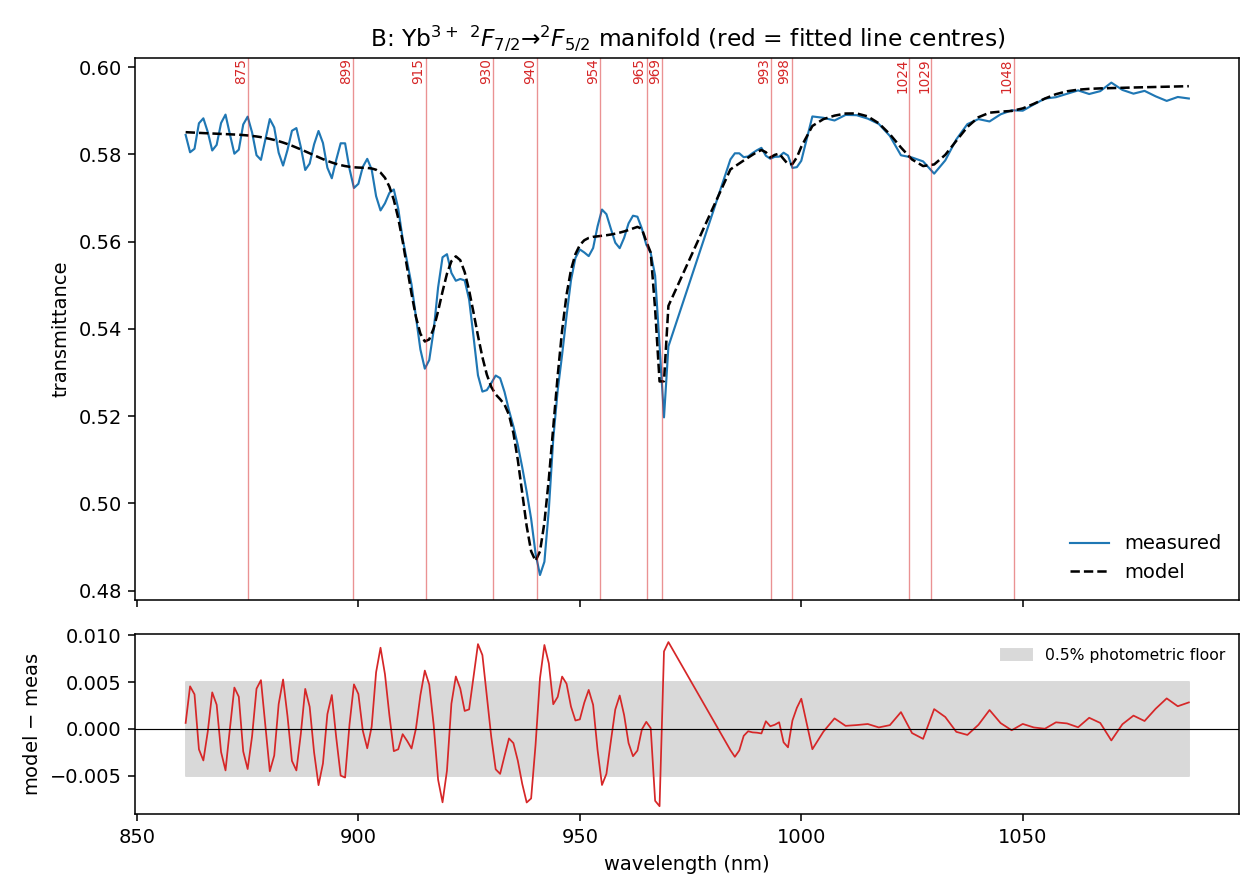
\includegraphics[width=0.92\textwidth]{fig_B_yb_band.png}
\caption{The Yb$^{3+}$ ${}^2F_{7/2}\!\to{}^2F_{5/2}$ manifold. Red lines mark
the \emph{predicted} centres. The model reproduces the $915$\,nm line, the
$921$\,nm peak between components, the $930$\,nm vibronic shoulder, the
$941$\,nm pump band, the sharp $969$\,nm zero-phonon line and the $997/1029$\,nm
hot bands. Lower panel: residual against the $0.5\%$ photometric floor (grey);
the regular oscillation below $950$\,nm is instrumental (Sec.~\ref{sec:dips}),
not material, and is deliberately not fitted.}
\end{figure}

\subsection{Fit quality}

\begin{center}\small
\begin{tabular}{@{}lcc@{}}
\toprule
Transmittance residual, $880$--$1080$\,nm & RMS & max \\
\midrule
3 broad Gaussians (first attempt) & 0.0087 & 0.0198\\
8 lines, centres free & 0.0026 & 0.0060\\
\textbf{13 lines, centres fixed at Stark values} & \textbf{0.0036} & \textbf{0.0093}\\
\bottomrule
\end{tabular}
\end{center}

The free-centre model scores marginally better but is \emph{not physical}: its
lines sit where the residual happens to be, not where Yb$^{3+}$ has transitions.
The fixed-centre model is the one to quote.

\subsection{Cross-validation}

Sample A was fitted from transmittance alone with $n$ frozen at B's
reflection-derived dispersion. It reproduces B's oscillator strengths to
$0.1$--$0.9\%$:

\begin{center}\small
\begin{tabular}{@{}lrr@{}}
\toprule
Line & B ($R+T$) & A ($T$ only)\\
\midrule
$915.2$\,nm & $1.919\times10^{-5}$ & $1.920\times10^{-5}$\\
$940.4$\,nm & $3.722\times10^{-5}$ & $3.693\times10^{-5}$\\
$954.5$\,nm (ZPL$+150$) & $1.462\times10^{-5}$ & $1.449\times10^{-5}$\\
$968.5$\,nm (ZPL) & $2.092\times10^{-5}$ & $2.090\times10^{-5}$\\
Scattering $C$, $p$ & $3.505$, $0.110$ & $3.530$, $0.131$\\
\bottomrule
\end{tabular}
\end{center}

Since the two samples were measured independently and A's fit never sees
reflection data, this is a genuine consistency check rather than a restatement
of the same numbers.

\begin{figure}[htbp]
\centering
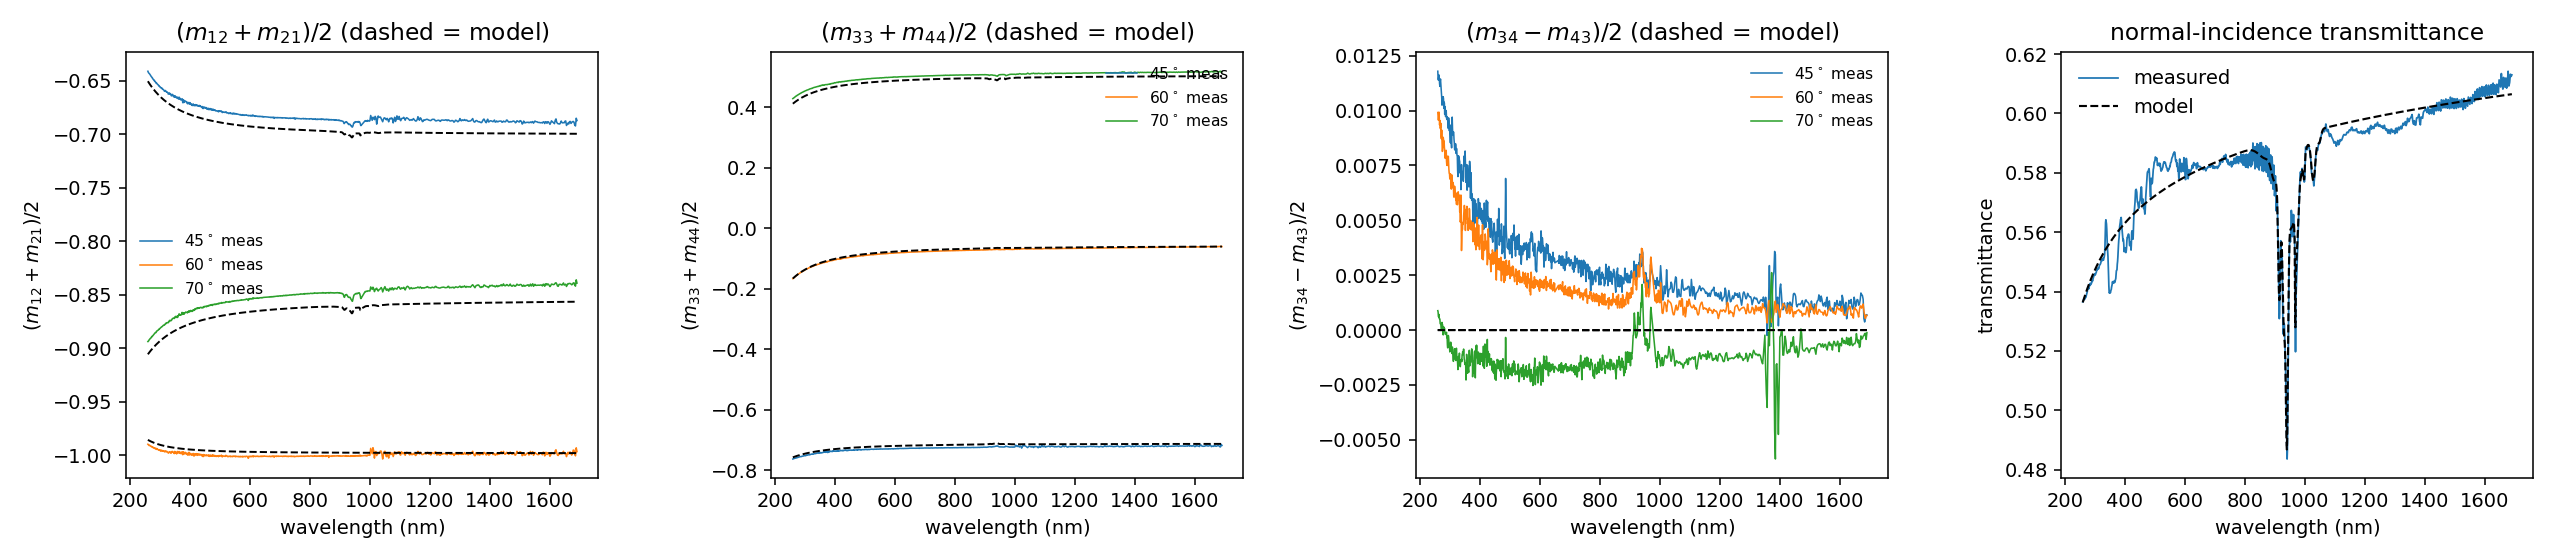
\includegraphics[width=\textwidth]{fig_B_fit_vs_data.png}
\caption{Measured (solid) and modelled (dashed) symmetrised Mueller elements at
three angles of incidence, and the normal-incidence transmittance. The
$s_{34}$ panel shows the one systematic residual the isotropic model does not
capture (Sec.~\ref{sec:limits}).}
\end{figure}

\section{Diagnostics: how the model was falsified and corrected}

This section records the tests that changed the analysis. Each was prompted by a
residual the model could not explain.

\subsection{Which transmission dips are real}
\label{sec:dips}

The measured transmittance contains \textbf{41 dips} with prominence
$>0.004$. Fitting oscillators to all of them would have injected fictitious $k$
and, through Eq.~\eqref{eq:kk}, corrupted $n$. They therefore had to be
classified first.

\paragraph{The test.} Reflection was acquired on 2026-06-30 and transmission on
2026-06-18. Genuine absorption raises $k$, which attenuates the backside beam and
so \emph{must} appear in the reflection Mueller matrix and in the
depolarisation. An artefact confined to the transmission channel will not.
Correlating the transmittance ripple against independently measured reflection
observables:

\begin{center}\small
\begin{tabular}{@{}lccl@{}}
\toprule
Band & corr($T$, depol) & corr($T$, $s_{12}$) & Verdict\\
\midrule
$300$--$500$\,nm & $-0.09$ & $+0.04$ & instrumental\\
$500$--$700$\,nm & $-0.06$ & $+0.08$ & instrumental\\
$700$--$900$\,nm & $+0.05$ & $-0.22$ & instrumental\\
$\mathbf{900}$--$\mathbf{1060}$\,\textbf{nm} & $\mathbf{+0.34}$ & $\mathbf{-0.42}$ & \textbf{real absorption}\\
$1100$--$1690$\,nm & $+0.06$ & $+0.20$ & instrumental\\
\bottomrule
\end{tabular}
\end{center}

Only the Yb manifold is material. The remaining $\sim30$ dips --- at $349$,
$403$, $467$, $486$, $544$, $581$, $602$, $611$, $756$\,nm, the dense
$800$--$880$\,nm series, $1105$ and $1527$\,nm --- live purely in the
transmission channel and are not fitted.

\paragraph{A tempting but invalid argument.} Samples A and B reproduce this
ripple at $r=0.98$--$0.99$. That is \emph{not} evidence that it is real, because
both share the same instrument. Only the reflection cross-check settles it.

\paragraph{Alternatives excluded.} The $800$--$950$\,nm ripple is not a
detector-interleave artefact: the sign alternation of consecutive differences is
$41$--$44\%$ (random is $50\%$) and the even/odd sample offset is
$6\times10^{-5}$. Nor is it a single etalon: an FFT in wavenumber returns
mutually inconsistent optical paths ($151$, $2.8$, $15.9\ \mu$m) in different
bands.

\subsection{The detector mask was too wide}

The Si/InGaAs crossover was initially masked over $965$--$983$\,nm. That range
\emph{swallowed the real zero-phonon line}. Inverting the transmittance at known
$n$ shows $\ad$ rising smoothly to $0.48$ at $969$\,nm --- physical absorption
--- whereas only at $971$--$983$\,nm does the transmittance jump to
$0.60$--$0.68$, above the sample's own out-of-band baseline ($\approx0.58$) and
therefore unphysical.

With the ZPL masked out, the fit had no oscillator for the absorption climbing
into the mask and compensated with the spurious $52$\,nm-wide ``line'' at
$955$\,nm. Narrowing the mask to $971$--$983$\,nm and adding the ZPL$+150\
\mathrm{cm}^{-1}$ vibronic replica removed the artefact and brought the
$950$--$965$\,nm residual below the photometric floor.

\subsection{A parameter-aliasing bug}

The routine mapping parameter names to oscillator indices parsed
\texttt{gauss12\_amp} with \texttt{int(head[-1])} --- the trailing
\emph{character}. With ten or more oscillators this maps
\texttt{gauss10..gauss13} onto indices $0..3$, silently aliasing four parameters
onto four others.

Symptoms, all initially misread as physics: every uncertainty returned
\texttt{NaN} (singular Jacobian); amplitudes were driven to absurd values
($9.95\times10^{-4}$ against a bound, versus $\sim10^{-5}$ for real lines); and
convergence took $697$ function evaluations instead of $45$. The printed
per-line table looked plausible throughout, because it reads the model
dictionary directly and never saw the aliased vector. The index is now parsed
with a regular expression, and
\texttt{python fit/dispersion.py} contains a regression test that round-trips
$14$ oscillators through pack/unpack.

The general lesson: a reporting path that bypasses the code under test will hide
the bug it is meant to reveal.

\section{Reproduction}

\begin{verbatim}
python -m fit.run_fit --sample B --thickness 1.0   # full R(10 AOI) + T fit
python -m fit.run_fit --sample A                   # reuses B's dispersion
python -m fit.run_fit --list                       # incl. screened-out files
python -m fit.plot_fit --sample B                  # figures
python fit/dispersion.py                           # KK + pack/unpack self-tests
python fit/slab.py                                 # forward-model self-tests
\end{verbatim}

Outputs land in \texttt{fit/out/}: \texttt{fit\_*\_nk.csv} (per-wavelength
$n$, $k$, $\alpha$, $\ad$, modelled and measured observables),
\texttt{fit\_*\_model.json} (parameters, uncertainties, line assignments) and
the figures reproduced above.

\section{Limitations and next steps}
\label{sec:limits}

\begin{enumerate}
\item \textbf{Thickness.} Only $\ad$ is measured. Supplying a micrometer
      measurement converts every amplitude to an absolute cross-section.
\item \textbf{Residual anisotropy.} $s_{34}$ shows a systematic rise towards the
      blue, $\approx0.012$ at $260$\,nm decaying to $\approx0.002$ in the NIR,
      which an isotropic model predicts as zero. Capturing it requires a
      uniaxial substrate; the implied $\Delta n$ is $\sim10^{-3}$.
\item \textbf{Two widths sit at bounds} ($875.1$\,nm upper, $965.1$\,nm lower);
      their uncertainties are not meaningful.
\item \textbf{Samples 5\,\% and 10\,\% must be re-measured.} Their transmission
      files are corrupt and the 5\,\% reflection scans show no polarisation
      change at $30^\circ$--$50^\circ$, indicating a failed alignment.
\item \textbf{Absolute Yb concentration} is not determined here; the oscillator
      strengths are per unit thickness and would need a calibrated
      cross-section, or a known reference sample, to convert to ion density.
\end{enumerate}

\begin{thebibliography}{9}
\bibitem{zelmon} D.~E.~Zelmon, D.~L.~Small and R.~Page,
  ``Refractive-index measurements of undoped yttrium aluminum garnet from
  0.4 to 5.0 $\mu$m,'' \emph{Appl.\ Opt.} \textbf{37}, 4933 (1998).
\bibitem{fan} T.~Y.~Fan \emph{et al.},
  ``Spectroscopy and diode laser-pumped operation of Tm,Ho:YAG'' and related
  Yb:YAG crystal-field analyses, \emph{IEEE J.\ Quantum Electron.}
  \textbf{24}, 924 (1988).
\bibitem{jellison} G.~E.~Jellison and F.~A.~Modine,
  ``Parameterization of the optical functions of amorphous materials in the
  interband region,'' \emph{Appl.\ Phys.\ Lett.} \textbf{69}, 371 (1996).
\bibitem{fujiwara} H.~Fujiwara, \emph{Spectroscopic Ellipsometry: Principles and
  Applications}, Wiley (2007) --- incoherent substrate treatment and Mueller
  formalism.
\bibitem{aspnes} D.~E.~Aspnes, ``Optical properties of thin films,''
  \emph{Thin Solid Films} \textbf{89}, 249 (1982) --- effective-medium theory.
\end{thebibliography}

\end{document}
